% !TEX TS-program = pdflatex
% !TEX encoding = UTF-8 Unicode

% This is a simple template for a LaTeX document using the "article" class.
% See "book", "report", "letter" for other types of document.

\documentclass[12pt]{article} % use larger type; default would be 10pt

\usepackage[utf8]{inputenc} % set input encoding (not needed with XeLaTeX)

%%% Examples of Article customizations
% These packages are optional, depending whether you want the features they provide.
% See the LaTeX Companion or other references for full information.

%%% PAGE DIMENSIONS
\usepackage{geometry} % to change the page dimensions
\geometry{a4paper} % or letterpaper (US) or a5paper or....
\geometry{margin=1cm} % for example, change the margins to 2 inches all round
% \geometry{landscape} % set up the page for landscape
%   read geometry.pdf for detailed page layout information

\usepackage{graphicx} % support the \includegraphics command and options

% \usepackage[parfill]{parskip} % Activate to begin paragraphs with an empty line rather than an indent

%%% PACKAGES
\usepackage{booktabs} % for much better looking tables
\usepackage{array} % for better arrays (eg matrices) in maths
\usepackage{paralist} % very flexible & customisable lists (eg. enumerate/itemize, etc.)
\usepackage{verbatim} % adds environment for commenting out blocks of text & for better verbatim
\usepackage{subfig} % make it possible to include more than one captioned figure/table in a single float
% These packages are all incorporated in the memoir class to one degree or another...

%%% HEADERS & FOOTERS
\usepackage{fancyhdr} % This should be set AFTER setting up the page geometry
\pagestyle{fancy} % options: empty , plain , fancy
\renewcommand{\headrulewidth}{0pt} % customise the layout...
%\lhead{}\chead{}\rhead{}
%\lfoot{}\cfoot{}\rfoot{}

%%% SECTION TITLE APPEARANCE
\usepackage{sectsty}
\allsectionsfont{\sffamily\mdseries\upshape} % (See the fntguide.pdf for font help)
% (This matches ConTeXt defaults)

%%% ToC (table of contents) APPEARANCE
\usepackage[nottoc,notlof,notlot]{tocbibind} % Put the bibliography in the ToC
\usepackage[titles,subfigure]{tocloft} % Alter the style of the Table of Contents
\renewcommand{\cftsecfont}{\rmfamily\mdseries\upshape}
\renewcommand{\cftsecpagefont}{\rmfamily\mdseries\upshape} % No bold!

%%% END Article customizations

\newcommand{\aufgabe}[1]{{\huge Statistik Übung \underline{Aufgabe #1}}\\[3.5ex]  } 
\usepackage{amsmath}
\usepackage{amssymb}
%%% The "real" document content comes below...

\begin{document}
\aufgabe{21}
Aufgabenstellung: \\
Sie spielen mit einem (stochastisch unbedarften) Kollegen um die letzte Flasche Bier. \\
Sie werfen abwechselnd mit einem Würfel. Derjenige, der zuerst eine 6 würfelt, gewinnt. \\
Sollten Sie anfangen mit Würfeln oder dem Kollegen den ersten Wurf überlassen? \\
Mit welcher Wahrscheinlichkeit gewinnen Sie? \\[0.5cm]
Lösung: \\
Wir sollten beginnen und gewinnen mit einer Wahrscheinlichkeit von $\frac{6}{11} = 54,5\% $\\[0.5cm]
Begründung: \\
Zufallsvariable $X$: Beim $X$-ten Wurf kommt das erste Mal eine sechs. $X \sim \text{Geo}(\frac{1}{6})$\\
Indikator-Zufallsvariable $E$: Es kommt bereits bei den ersten beiden Versuchen eine sechs. \\
Indikator-Zufallsvariable $S$: $X$ ist ungerade, also wir gewinnen. \\
$P(S=1 ~ | ~ E=1) = \frac{P(S=1, E=1)}{P(E=1)} = \frac{P(X=1)}{P(X \leq 2)} = \frac{1/6}{1-(5/6)^2} = \frac{6}{11}$ \\
Wegen der Gedächtnislosigkeit der geometischen Verteilung gilt, dass $S$ und $E$ unabhängig sind und somit $P(S=1) = P(S=1 | E=1)$\\
Begründung Unabhängigkeit: $P(S=1) = P(X ~ \text{ungerade}) = $ \\ 
$ ~~ = \sum_{2 \nmid x \wedge x \in \mathbb{N}} P(X=x) = $ \hspace{3cm}\small{ (immer erfüllte Nebenbedingung)}\\
$ ~~ = \sum_{2 \nmid x \wedge x \in \mathbb{N}} P(X=x ~ | ~ X \geq 1) = $ \hspace{2cm}\small{ (Gedächtnislosigkeit)}\\
$ ~~ = \sum_{2 \nmid x \wedge x \in \mathbb{N}} P(X=x+2 ~ | ~ X \geq 1+2) = $ \hspace{1cm}\small{ (Summen-Index-Shift um 2)}\\
$ ~~ = \sum_{2 \nmid x \wedge x \in \mathbb{N}_{x\geq 3}} P(X=x ~ | ~ X > 2) = P(X ~ \text{ungerade} \wedge X > 2 ~ | ~ X > 2) = $\\
$ ~~ = P(X ~ \text{ungerade}, E = 0 ~ | ~ E = 0) = P(S=1, E=0 ~ | ~ E=0) = P(S=1 ~ | ~ E=0)$\\[1ex]
\- \dotfill
\\[4ex]
\aufgabe{22}
Aufgabenstellung: \\
Geben Sie zu den folgenden Merkmalen an, welche Ausprägungen sie besitzen und ob sie nominal, ordinal oder metrisch (= numerisch) sind. \\[0.5cm]
\begin{tabular}{|l l |c|c|c| l |}
\hline 
~ & Merkmal                                                     & nom. & ord. & metr. & Ausprägungen \\ \hline \hline
a & Wasserhärtegrad                                       & - & x & - & weich, mittel, hart \\ \hline
b & Lebensalter von Elefanten                         & - & - & x & Alter in Jahren $\in \mathbb{N}_0$ \\ \hline
c & Parteizugehörigkeit                                     & x & - & - & keine, Partei1, Partei2, ... \\ \hline
d & Stammumfänge von zehnjährigen Fichten & - & x & x & Umfang in mm $\in \mathbb{R}_{0}^{+}$ oder Kategorien \\ \hline
e & Gewichtsklasse von Eiern                           & - & x & - & A, B, C, ... \\ \hline
f & Anzahl der Blütenblätter von B-w-röschen & - & - & x & Anzahl $\in \mathbb{N}_0$ \\ \hline
g & Temperatur                                                & - & x & x & kalt, warm, heiß oder in $^\circ$C $\in \mathbb{R}$ \\ \hline
h & Verkehrsdichte auf einer Straße                & - & x & x & frei, zäh, Stau oder in Autos / l / t  $\in \mathbb{N}_0$ \\ \hline
i & Berufswunschangaben von Abiturenten     & x & - & - & Pilot, Manager, ... \\ \hline
j & Noten                                                          & - & x & x & als enum oder int oder float \\ \hline  
\end{tabular}

\newpage
\aufgabe{23}
Aufgabenstellung: \\
Es soll eine neugezüchtete Kartoffelsorte gestetet werden. Dazu wird ein Testfeld ausgewählt, das auf der gesamten Fläche gleiche Wachstumsvoraussetzungen (Bodenqualität, Sonneneinstrahlung, ...) bietet. Nachdem eine gleichmäßige Pflege der Pflanzen erfolgte (Bewässerung, Düngung, ...) wurde von der ersten Ernte auf dem Versuchsfeld eine Stichprobe entnommen, die die folgende Urliste lieferte: \\
\begin{tabular}{| l || c | c | c | c | c | c | c | c | c | c |}
\hline
$j$ & $1$ & $2$ & $3$ & $4$ & $5$ & $6$ & $7$ & $8$ & $9$ & $10$ \\ \hline
$x_j$ & $132$ & $145$ & $172$ & $151$ & $152$ & $136$ & $143$ & $112$ & $159$ & $152$ \\ \hline
\end{tabular}\\[0.4cm]
a) Bestimmen Sie die geordnete Stichprobe\\
\begin{tabular}{| c | c | c | c | c | c | c | c | c | c |}
\hline
$x_{(1)}$ & $x_{(2)}$ & $x_{(3)}$ & $x_{(4)}$ & $x_{(5)}$ & $x_{(6)}$ & $x_{(7)}$ & $x_{(8)}$ & $x_{(9)}$ & $x_{(10)}$ \\ \hline
$112$ & $132$ & $136$ & $143$ & $145$ & $151$ & $152$ & $152$ & $159$ & $172$ \\ \hline
\end{tabular}\\[0.4cm]
b) Klassenhistogramm\\
\begin{tabular}{| c | c | c | c | c | c | c | c | c | c |}
\hline
Klasse                       & $]110, 140]$ & $]140, 150]$ & $]150, 180]$ \\ \hline
Anzahl Datensätze   & $3$ & $2$ & $5$ \\ \hline
Klassenbreite            & $30$ & $10$ & $30$ \\ \hline
Hoch                         & $60$ & $120$ & $100$ \\ \hline
\end{tabular}\\[0.4cm]
c) empirische Verteilungsfunktion unklassiert und d) klassiert \\
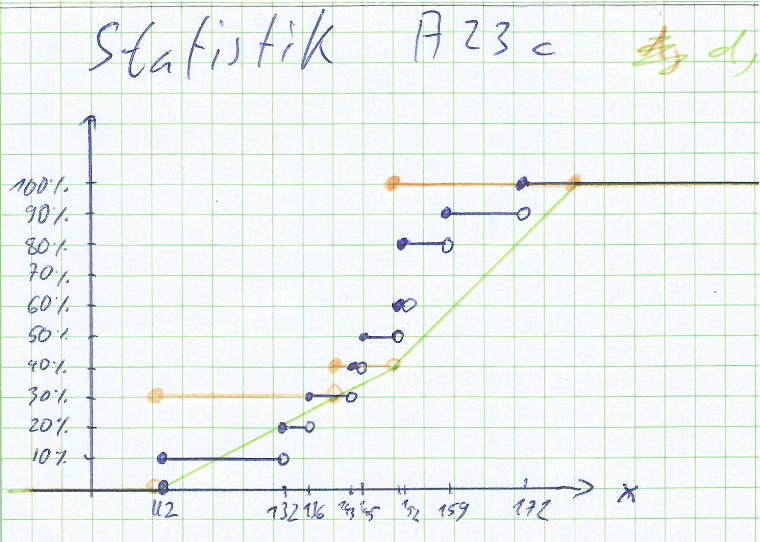
\includegraphics{A23c.pdf} \\[0.4cm]
e) arithmetisches Mittel $\overline{x} = \frac{\sum_{i=1}^{10}{x_i}}{10} = \frac{1454}{10} = 145,4 $\\[0.4cm]
f) Median $x_{0,5} = \frac{x_{(5)} + x_{(6)}}{2} = \frac{145 + 151}{2} = 148$ \\[0.4cm]
g) unteres Quartil $x_{0,25} = x_{(3)} = 136$ \\[0.4cm]
h) oberes Quartil $x_{0,75} = x_{(8)} = 152$ \\[0.4cm]
i) Quartilsabstand $x_{0,75} - x_{0,25} = 152 - 136 = 16$ \\[0.4cm]
j) $30\%\text{-Quantil} ~~ x_{0,3} \in [x_{(3)}, x_{(4)}] = [136, 143]$ \\[0.4cm]
\newpage
\aufgabe{24}
Anzahl Bücher: $90 + 55 = 145$ \\
Median der Seitenzahl: $x_{0.5} \in [350, 450]$ \\
Mittelwert der Seitenzahl: $\overline{x} = \frac{400 * 90 + 500 * 55}{90+55} = \frac{63.500}{145} = 437,9$ \\ 
$95\%\text{-Quantil} ~~ x_{0,95} \in [710, 800]$ \\[1ex]
\- \dotfill 
\\[4ex]
\aufgabe{25}
a) Binomialverteilung $B(100M, p)$ mit $p = \frac{1}{\binom{49}{6}} = \frac{1}{13.983.816} = 71,5 *10^{-9}$ \\
b) Binomialverteilung mit grossem $n$ und kleinem $p \Longrightarrow $  Poissonverteilung geeignet. $\alpha = np = 7,15$  \\
c) 
\end{document}
